\chapter{Introduction}

\section{Introduction}\label{sec:intro}

The mission of particle physics is to increase our understanding of the most fundamental constituents of our universe and their interactions. These efforts have arguably been going on since the era of the Greek philosophers, who classified all matter into the elemental categories of earth, air, wind, and fire. As the centuries progressed, our knowledge of the nature of the universe has been refined as new theories were proposed to explain the phenomena we observe in nature, and, at the same time, more and more sophisticated experiments were designed to test them. Particle physicists are broadly divided into two sub-fields: theorists and experimentalists. Theorists seek to develop models that offer a more complete explanation of particle interactions, and experimentalists are tasked with validating these models. Efforts in particle theory in the late-20th century culminated in the Standard Model (SM) of particle physics, which has proven to be tremendously successful at describing a large number of observed particle phenomena (some which have been accurately validated to one part in ten billion!).

The SM is not without its deficiencies, however. Today, there remain many open questions in particle physics that are not sufficiently (or at all) addressed by the SM. To name just a few: 

Why is there more matter than antimatter in the universe?
What is dark matter?
What is dark energy?
Can the strong iteraction be unified with the electroweak interaction?
Why is the Higgs mass 125 GeV and not at the Planck scale?

Attempts to answer these questions require new theories modifying and building on the SM. These theories must then be tested, which is where the experimentalists come in. While the SM was perhaps the crowning achievement of high energy theory in the twentieth century, the Large Hadron Collider (LHC) is arguably the most noteworthy undertaking in high energy experiment in the twenty-first. Located in Geneva, Switzerland at the European Organization for Nuclear Research (CERN, from the French ``Conseil Européen pour la Recherche Nucléaire"), the LHC is the highest-energy particle collider ever built and has been an invaluable tool in the quest to validate theories of new physics.

This thesis presents an effort to use one of the primary experiments on the LHC, the Compact Muon Solenoid (CMS), to search for a new particle, called the \emph{$Z^\prime$}, predicted by many such ``Beyond Standard Model" (BSM) theories. Part I will lay the groundwork, offering an overview of the SM and the modifying theories which predict the $Z^\prime$'s existence. Part II will discuss the tools used in the search: the LHC, the CMS experiment, and the substantial computing resources needed to conduct a full search for new physics. Part III will discuss the search during the 2012 data-taking run at the LHC, and Part IV will discuss the most recent search conducted during the 2015 run. Part V will offer an overview of future possibilities in this search effort as well as concluding remarks.

%\part{\huge Part I}

\chapter{The Standard Model}


As mentioned, the Standard Model (SM) of particle physics is the set of theories describing subatomic particles and their interactions according to the electromagnetic, weak, and strong forces. Describing these interactions individually are the theory of quantum electrodynamics (QED, electromagnetic), electroweak theory (EW, weak and elecromagnetic), and the theory of quantum chromodynamics (QCD, strong). These individual theories combine to form the symmetry group describing the SM:

$$SU(3)_{C} \times SU(2)_{L} \times U(1)_{Y}$$

\noindent\ where $SU(3)_{C}$ is the symmetry group describing QCD, while $SU(2)_{L} \times U(1)_{Y}$ together are the symmetry groups describing electroweak theory, the unification of the electromagnetic and weak interactions.

This chapter will begin with an overview of the fundamental particles in the SM, and then will provide a brief discussion of each of the constituent theories listed above. It will conclude with additional sections on specific elements of the SM which are especially relevant to searches for new physics at hadron colliders.

\section{Particles of the Standard Model}

Shown in Figure~\ref{fig:StandardModel}, the particles included the SM are believed to be fundamental (that is, they cannot be broken down into smaller constituent particles). Broadly, these particles can be divided into spin-1/2 particles, known as fermions, and integer-spin particles, known as bosons. 

\begin{figure}
\centering
  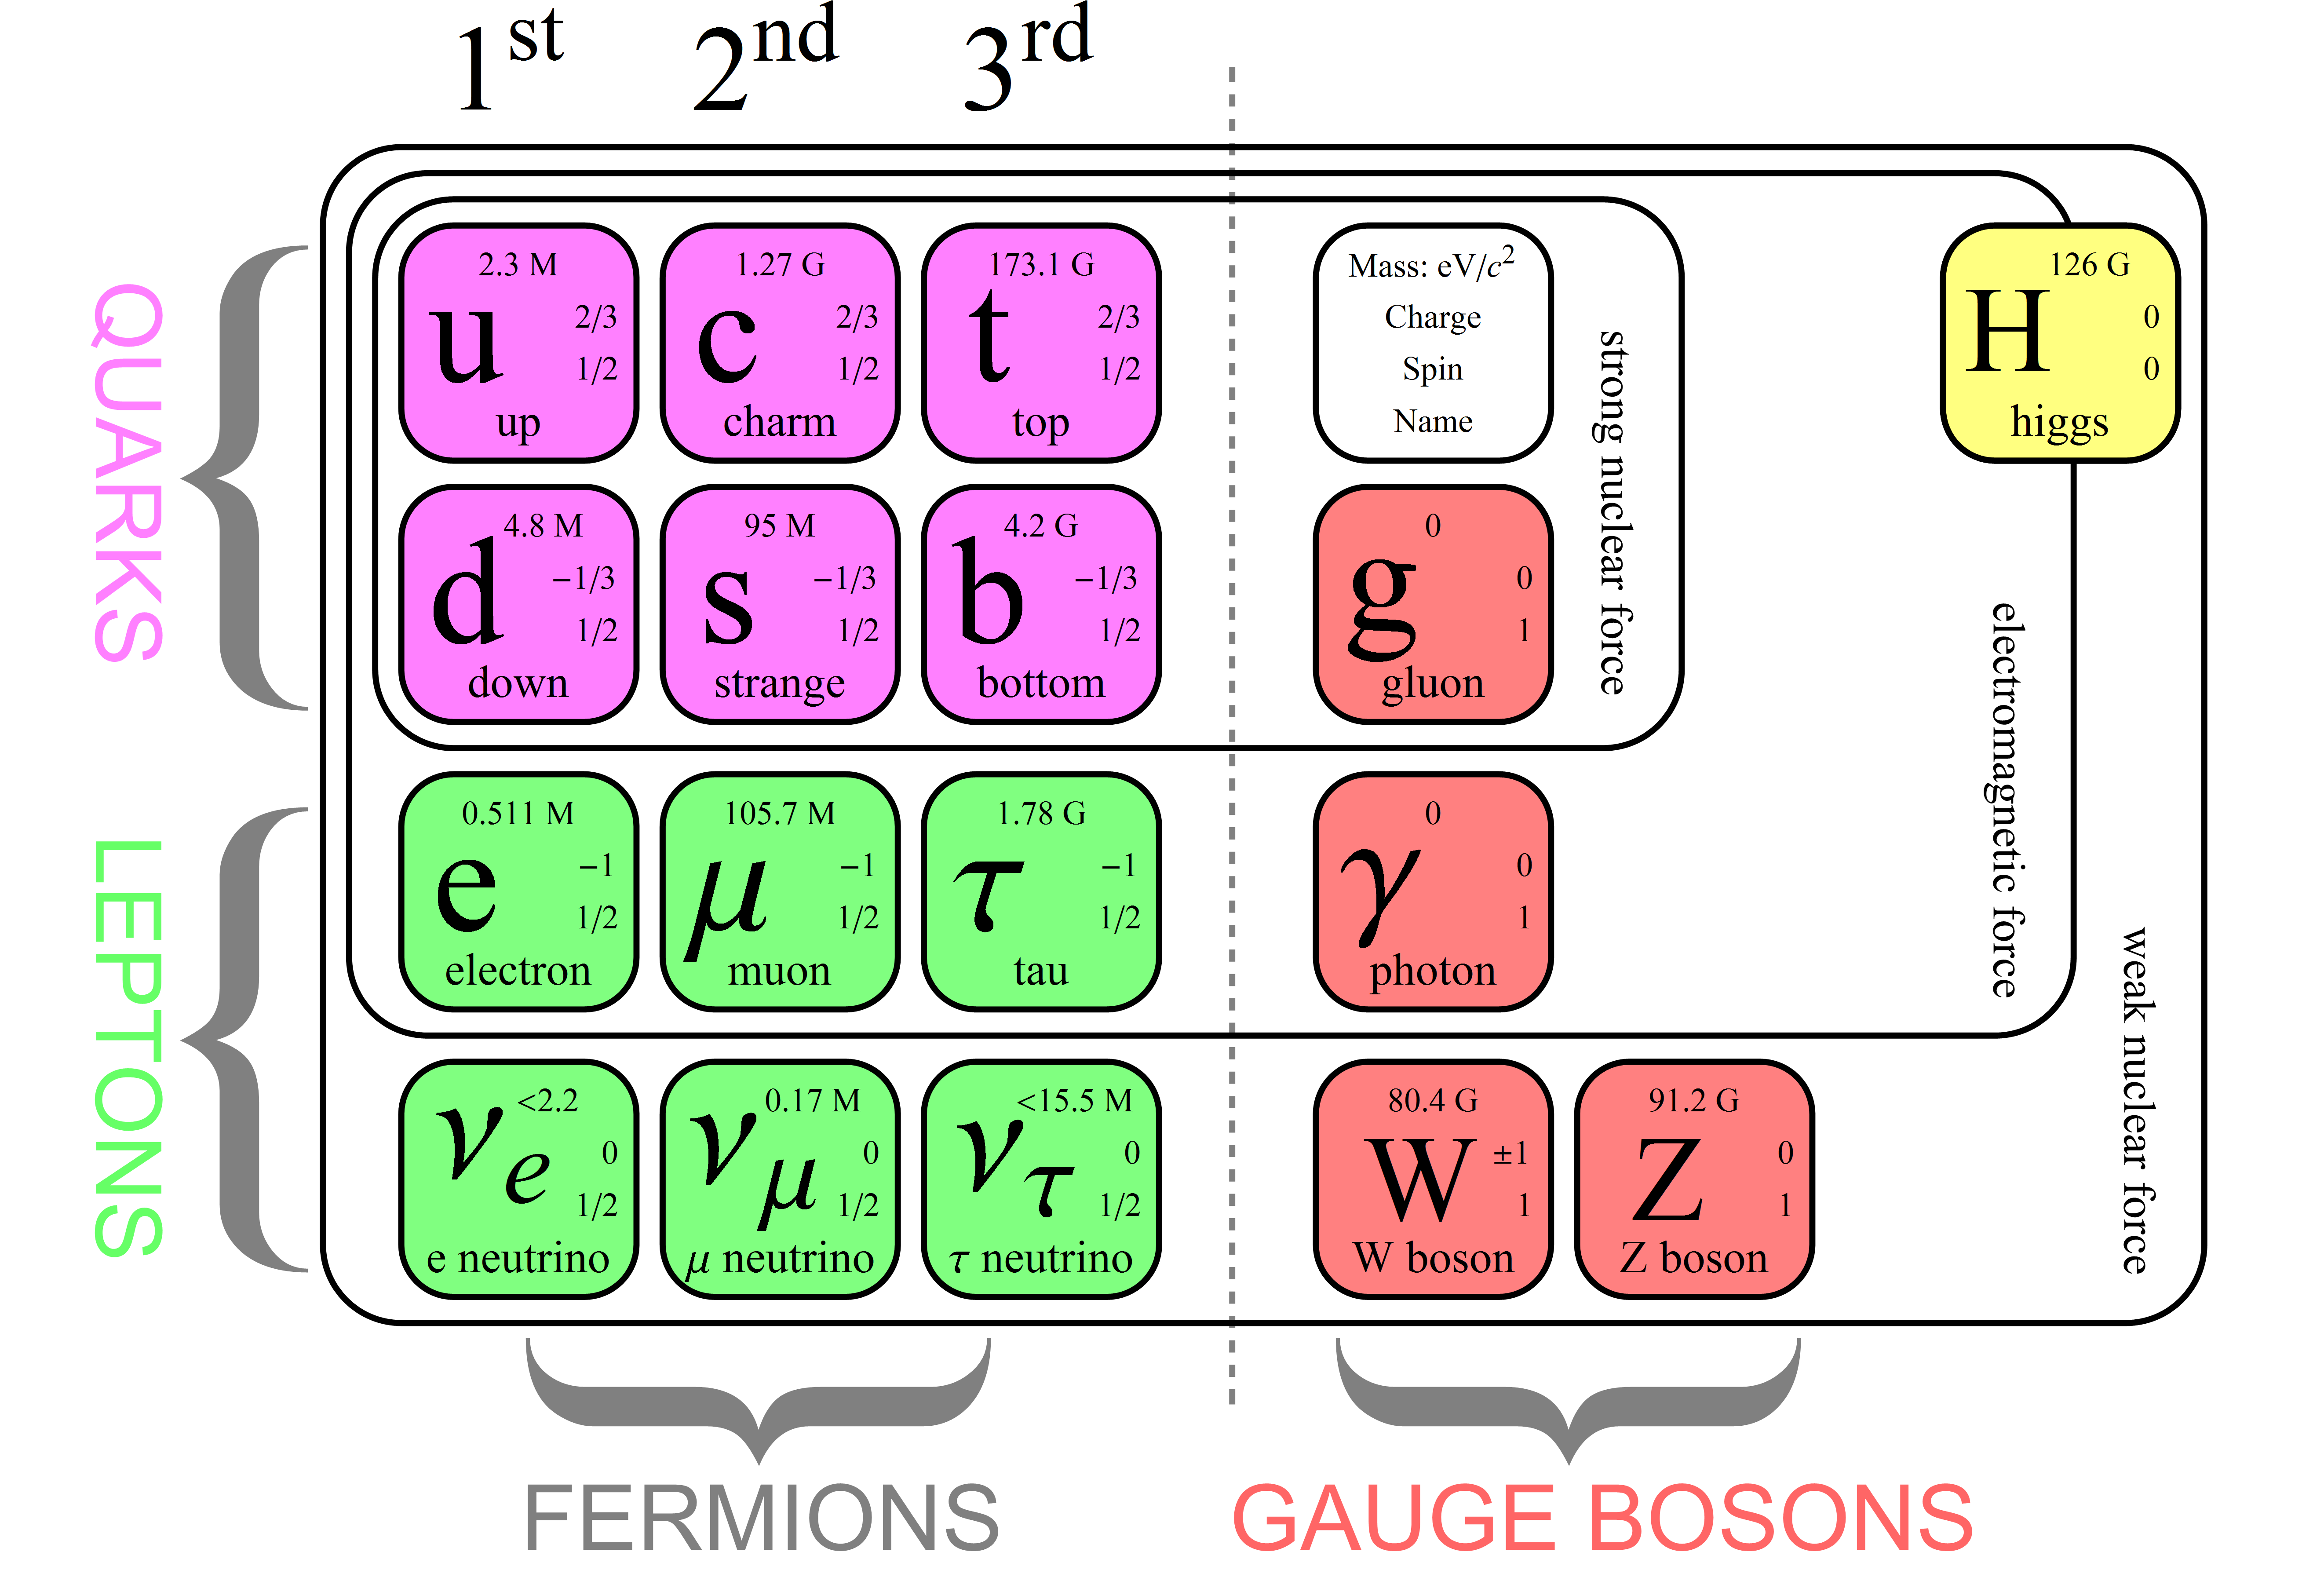
\includegraphics[width=0.4\textwidth]{figures/StandardModel.png}
  \caption{\label{fig:StandardModel} Table showing the quarks, leptons, and gauge bosons (force carriers) in the SM as well as the Higgs boson\cite{StandardModelTable}}
\end{figure}


Fermions make up the matter of our universe. They are further divided into quarks and leptons. Quarks combine with other quarks to form \textit{hadrons}. Hadrons are divided into \textit{baryons} and \textit{mesons}. Baryons are three-quark states such as the protons and neutrons which form atomic nuclei. Mesons are quark-antiquark pairs such as pions and kaons. Quarks have electric charge and interact via the electromagnetic and weak forces, and they also have color charge, meaning they interact via the strong force as well. This strong force is what keeps baryons and mesons held together and will be discussed further in the section on QCD. Quarks are divided into pairs of positive and negative charge across three ``generations" of increasing mass. In each pair, the positively-charged quark has electric charge +2/3 and the negatively-charged quark has electric charge -1/3. The first generation consists of the positively-charged \textit{up (u)} quark and the negatively-charged \textit{down (d)} quark. These are the quarks most commonly found in matter as they make up protons and neutrons in matter as well as the pions. The second generation consists of the positively-charged \textit{charm (c)} quark and the negatively-charged \textit{strange (s)} quark. These quarks form more exotic hadrons such as kaons and lambdas. The third generation consists of the positively-charged \textit{top (t)} quark and the negatively-charged \textit{bottom (b)} quark. These are quite heavy, quite short-lived quarks which are rarely found in bound states.

While the quarks interact via both the strong and electroweak forces, the leptons only experience the electroweak interaction. The nature of this interaction will be discussed further in the sections on QED and EW theory. Like the quarks, the leptons are divided into three generations. Each generation consists of a negatively-charged particle with charge -1, and a companion neutrino which is electrically-neutral. The first generation consists of the electron (\textit{e}), the most commonly-found lepton forming shells around nuclei to create atoms and being responsible for electric current, and its corresponding neutrino, the electron neutrino (\textit{$\nu_{e}$}). The second generation consists of the muon (\textit{$\mu$}) and its corresponding neutrino, the muon neutrino (\textit{$\nu_{\mu}$}). Muons are heavier than electrons and decay primarily into an electron, a muon neutrino, and an electron antineutrino. The mean lifetime of a muon is about 2 $\mu$s (in the reference frame of the muon). The third generation consists of the tau (\textit{$\tau$}) and its corresponding neutrino, the tau neutrino (\textit{$\nu_{\tau}$}). Taus are heavier still and can decay either leptonically or hadronically. In both cases, the tau decays directly into a tau neutrino and a $W$ boson matching the sign of the tau. In the hadronic case, the $W$ decays into a quark-antiquark pair which quickly hadronizes into jets, and in the leptonic case, the $W$ decays into either an electron and electron antineutrino or a muon and a muon antineutrino.  The mean lifetime of a tau is about $3 \times 10^{-13}$s (in the reference frame of the tau).\cite{pdg}

The bosons act as the force carriers of the SM. The photon (\textit{$\gamma$}) mediates the electromagnetic interaction, the gluon (\textit{g}) mediates the strong interaction, and the W and Z bosons mediate the weak interaction. The W can have electric charge +1 (\textit{$W^{+}$}) or -1 (\textit{$W^{-}$}), while the Z, photon, and gluon are all electrically neutral. The W and Z are also massive, while the photon and gluon are each massless. These bosons, known as guage bosons or vector bosons, each have spin 1. The final boson, the scalar (spin 0) Higgs boson, is the final boson in the Standard Model and is responsible for mediating the Higgs field (discussed further in the section on the Higgs mechanism).

\section{Quantum Electrodynamics}

Quantum electrodynamics (QED) describes the interactions between particles having electric charge and the photons which mediate the electromagnetic force. A massive, unconstrained, fermionic field $\psi(x)$ with mass m (such as an electron) may be described according to the Dirac Langrangian\cite{srednicki}:
\begin{equation}
\mathcal{L}_{\text{Dirac}} = i\bar{\psi}\gamma^{\mu}\left(\partial_{\mu} + ieA_{\mu}\right) - m\bar{\psi}\psi
\end{equation}
where the $\gamma^{\mu}$ are Dirac matrices representing Lorentz transformations on the Dirac spinors $\psi$, and the $A_{\mu}$ correspond to the photon field. This Lagrangian corresponds to observable fields, so it must be invariant under gauge transformations. $\psi(x)$ is invariant under Lorentz transformations, and we define it to be invariant under the transformation
\begin{equation}
\psi(x) \to e^{ie\alpha(x)}\psi(x)
\end{equation}
where $e$ is the electron charge ($\approx 1.6 \times 10^{-19}$ Coulombs) and $\alpha(x)$ is some position-dependent angle.

To transform $\psi(x)$ in position to $\psi(y)$, we define the scalar operator $U(x, y)$ such that
\begin{equation}
\psi(y) = U(x, y)\psi(x)
\end{equation}

\noindent If we take the transformation to be infinitesimally small, we have
\begin{equation}
y = x + \epsilon\ n^{\mu}
\end{equation}

\noindent If we expand this, we get
\begin{equation}
U(x, x + \epsilon\ n^{\mu}) = 1 - \epsilon\ en^{\mu}A_{\mu} + O(\epsilon^{2}).
\end{equation}

\noindent In order for the Lagrangian to remain invariant, we must have
\begin{equation}
A_{\mu}(x) \to A_{\mu}(x) - \frac{1}{\epsilon}\partial_{\mu}\alpha(x).
\end{equation}

\noindent Now, if we define
\begin{equation}
D_{\mu} \equiv \partial_{\mu} + ieA_{\mu}
\end{equation}

\noindent we can construct the commutator

\begin{equation}
\left[D_{\mu}, D_{\nu}\right]\psi(x) = \left(D_{\mu}D_{\nu} - D_{\nu}D_{\mu}\right)\psi(x)
= ie\left(\partial_{\mu}A_{\nu} - \partial_{\nu}A_{\mu}\right)\psi(x) \equiv ieF_{\mu\nu}\psi(x)
\end{equation}

\noindent which allows our Lagrangian to be fully gauge invariant. Note that there is no mass term $A_{\mu}A_{\mu}$, ensuring that the photon is massless. Putting everything together, we arrive at the final Lagrangian for QED~\cite{halzen}:

\begin{equation}
\mathcal{L}_{\text{QED}} = \bar{psi}\left(i\gamma^{\mu}D_{\mu} - m\right)\psi - \frac{1}{4}F_{\mu}{\nu}F^{\mu}{\nu}.
\end{equation} 

\noindent A typical QED interaction, an electron-positron pair annihilating into a photon which then decays into another electron-positron pair, is shown in Figure~\ref{fig:FeynmanQED}.

\begin{figure}
\centering
  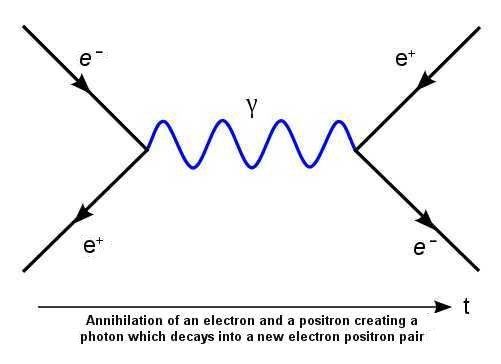
\includegraphics[width=0.4\textwidth]{figures/FeynmanQED.jpg}
  \caption{\label{fig:FeynmanQED} Typical QED interaction\cite{QEDFeynman}}
\end{figure}


\section{Electroweak Theory}
\label{sec:EW}

The weak force is responsible for radioactive decay and is mediated by the W and Z bosons. It is perhaps best understood in terms of its unification with electromagnetism known as Electroweak theory. Both quarks and leptons can interact via the weak force, with W and Z bosons decaying to both. 

The symmetry group of EW theory is $SU(2)_{L} \times U(1)_{Y}$, where $SU(2)_{L}$ is non-Abelian with generators $I_{i} = \sigma_{i}$ where $\sigma_{i}$ are the standard Pauli matrices, and where $U(1)_{Y}$ is Abelian with generator $Y/2 = Q - I_{3}$ where $Q$ is the electric charge. The corresponding gauge bosons are the $W_{1}$, $W_{2}$, and $W_{3}$ from $SU(2)_{L}$, and the $B$ from $U(1)_{Y}$ and are all massless. Through spontaneous symmetry breaking via the Higgs mechanism, these four massless bosons become the massive $W^{\pm}$ and $Z$ and the massless photon of the SM.

Before electroweak symmetry breaking, the EW Lagrangian is defined to be\cite{srednicki}

\begin{equation}
\mathcal{L}_{\text{EW}} = -\frac{1}{4}W^{i}_{\mu\nu}W^{\mu\nu}_{i} - \frac{1}{4}B_{\mu\nu}B^{\mu\nu} + \bar{f_{L}}\gamma^{\mu}\left(i\partial_{\mu} - \frac{g}{2}\sigma_{i}W^{i} - g^{\prime}\frac{Y}{2}B_{\mu}\right)f_{L} + 
\bar{f_{R}}\gamma^{\mu}\left(i\partial_{\mu} - g^{\prime}\frac{Y}{2}B_{\mu}\right)f_{R}
\end{equation}

\noindent where we define:

\begin{equation}
W^{i}_{\mu\nu} \equiv \partial_{\mu}W^{i}_{\mu} - \partial_{\nu}W^{i}_{\mu} - g\epsilon_{ijk}W^{j}_{\mu}W^{k}_{\nu}
\end{equation}

\noindent and

\begin{equation}
B_{\mu\nu} \equiv \partial_{\mu}B_{\nu} - \partial_{\nu}B_{\mu}.
\end{equation}

Here, $g$ and $g^{\prime}$ are the respective coupling constants for $SU(2)_{L}$ and $U(1)_{Y}$, and $f_{R}$ and $f_{L}$ represent right- and left-handed fermionic fields, respectively. ``Handedness", or helicity, is simply the dot product of the momentum and spin unit vectors of the particle. Right-handed particles have helicity +1, and left-handed particles have helicity -1.

After spontaneous symmetry breaking, the massless $W_{1}$ and $W_{2}$ combine to form the massive $W^{\pm}$ via the relation

\begin{equation}
W^{\pm} = \frac{1}{\sqrt{2}}\left(W_{1} \mp iW_{2}\right)
\end{equation}

\noindent and the massless $B$ and $W_{3}$ combine to form the massive $Z$ and massless photon via the relation
\begin{equation}
\begin{pmatrix}\gamma \\Z\end{pmatrix}=\begin{pmatrix}\cos \theta _{W}&\sin \theta _{W}\\-\sin \theta _{W}&\cos \theta _{W}\end{pmatrix}\begin{pmatrix}B\\W_{3}\end{pmatrix}
\end{equation}

\noindent where $\theta_{W}$ is the weak mixing angle, which defines the rotation by which spontaneous symmetry breaking transforms the $W_{1,2,3}$ and $B$ into the $W^{\pm}$, $Z$, and photon of the SM. In terms of the coupling constants of $SU(2)_{L}$ and $U(1)_{Y}$, the weak mixing angle may be defined as\cite{srednicki}:

\begin{equation}
\cos \theta_{W} = \frac{g}{\sqrt{g^{2} + g^{\prime2}}}
\end{equation}

\noindent and empirically as 

\begin{equation}
\cos \theta_{W} = \frac{m_{W}}{m_{Z}}.
\end{equation}~\cite{halzen}

\section{Quantum Chromodynamics}

Quantum chromodynamics (QCD) is the theory that describes the strong force. QCD introduces a new property, called ``color," that is only felt by particles which strongly interact. These particles are quarks ($q$, the constituents of baryons and mesons) and gluons ($g$, the mediator of the strong force). Particles can have color charge ``red", ``green", or ``blue" according to rotations in the group $SU(3)_{C}$, the portion of the SM relevant to QCD.

The generators of $SU(3)$ are eightfold, and can be used to represent the gauge transformation $U(\alpha)$:

\begin{equation}
U(\alpha) = e^{i\alpha_{j}}T^{j} \approx I + i\alpha_{j}T^{j} + O(\alpha^{2})
\end{equation}

\noindent They satisfy the commutation relation:

\begin{equation}
\left[T^{a}, T^{b}\right] = if^{abc}T^{c}
\end{equation}

\noindent where 

\begin{equation}
f^{abc} \equiv -2i\text{Tr}\left(T^{a}T^{b}T^{c} - T^{b}T^{a}T^{c}\right).
\end{equation}

\noindent We can write the Lagrangian of QCD as:

\begin{equation}
\mathcal{L}_{\text{QCD}} = -\frac{1}{4}F^{\mu\nu}_{\alpha}F^{\alpha}_{\mu\nu} + \bar{q}\left(i\gamma^{\mu}D_{\mu} - m\right)q - \frac{1}{2\xi}\partial_{\mu}A^{\alpha\mu}\partial_{\nu}A^{\alpha\nu} + \partial_{\mu}\bar{c}^{a}\left(\partial^{\mu}\delta^{ab} + g_{s}f_{abc}A^{c\mu}\right)c_{b}.
\end{equation}\cite{halzen}

\noindent Here, we define

\begin{equation}
D_{\mu} \equiv \partial_{\mu} + ig_{s}A^{\mu}_{a}T^{a}
\end{equation}

\noindent and

\begin{equation}
F^{\alpha}_{\mu\nu} \equiv \partial_{\mu}A^{\alpha}_{\nu} - \partial_{\nu}A^{\alpha}_{\mu} - g_{s}f^{abc}A^{b}_{\mu}A^{c}_{\nu}
\end{equation}

\noindent where $g_{s}$ is the coupling constant of the strong force and $A^{\mu}$ represents the gluon field. The first term in the Lagrangian represents the gluon propagator, but note that it also includes a gluon self-interaction. This is in contrast to the QED Lagrangian, which allows no photon self-interaction. Due to this, QCD in fact allows for a bound state made entirely of gluons known as a ``glueball," although none have been experimentally observed. The second term represents the quark-gluon interactions as well as the free quark propagator. The final two terms are required to keep the Lagrangian gauge-invariant.

No stable particle may have non-neutral overall color charge. Since quarks and gluons on their own have net color charge, they immediately pull quarks and gluons out of the vacuum in order to form color-neutral bound states. These bound states may either achieve color neutrality in the form of a quark-antiquark pair (e.g. red + antired = color-neutral), or as a three-quark baryon (red + green + blue = color-neutral). This process of pulling strongly-interacting particles out of the vacuum is called \textit{hadronization}. Hadronization occurs because the strong force is extremely short-ranged (on the order of a proton radius). As two color-charged particles are pulled apart, the energy required to keep them in a bound state satisfying color-neutrality increases rapidly. Very quickly, it becomes energetically favorable to pull a quark-antiquark pair out of the vacuum to form new color-neutral states. This requirement of color-neutrality is called \textit{color confinement}, and the property of the strong coupling strength increasing rapidly with distance is known as \textit{asymptotic freedom}~\cite{halzen}.


\section{Spontaneous Symmetry Breaking and the Higgs Mechanism}

Recall from ~\ref{sec:EW} that, although the gauge bosons of the electroweak interaction, the $W_{1,2,3}$ and the $B$, are required by gauge invariance to be massless, some of their SM counterparts, the $W^{\pm}$ and $Z$, are observed to be massive (80.4 GeV and 91.2 GeV, respectively). In order for these bosons to retain their mass without violating the gauge symmetry, the Higgs mechanism was introduced to explain this spontaneous symmetry breaking.

Developed by Peter Higgs in 1964, the Higgs mechanism introduces an extra potential term $V(\Phi)$ into the EW Lagrangian, where 

\begin{equation}
\Phi \equiv \begin{pmatrix}\phi^{+} \\ \phi^{0}\end{pmatrix}_{L}
\end{equation}

\noindent and

\begin{equation}
V(\Phi) \equiv \mu^{2}\Phi^{\dagger}\Phi + \lambda\left(\Phi^{\dagger}\Phi\right)^{2}.
\end{equation}

\noindent The total addition to the EW Lagrangian is of the form

\begin{equation}
\mathcal{L}_{Add} = D_{\mu}\Phi\ D^{\mu}\Phi - V(\Phi).
\end{equation}

Minimizing the potential $V(\Phi)$ in $\Phi$ gives the vacuum expectation value (VEV) of $\Phi$. If we choose $\mu^{2} < 0$, we arrive at multiple critical points in our minimization and a degenerate state is possible. The VEV takes the form

\begin{equation}
\braket{0|\Phi|0} = \begin{pmatrix}0 \\ \frac{\mu^{2}}{\sqrt{2}\lambda}\end{pmatrix}.
\end{equation}~\cite{srednicki}

This VEV has inifinite degenerate minima all with the same magnitude but different phase. Choosing one phase leads to spontaneous symmetry breaking, and the $W$ and $Z$ bosons acquire mass via\cite{halzen}

\begin{equation}
m_{W} = \frac{g}{2}\frac{|\mu^{2}|}{\lambda}
\end{equation}
\begin{equation}
m_{Z} = \frac{m_{W}}{\cos{\theta_W}}.
\end{equation}

The final piece of the SM, the Higgs boson, has a mass which is dependent entirely on the VEV:

\begin{equation}
m_H = sqrt{2|\mu^2|}.
\end{equation}

In July 2012, the Higgs boson was discovered concurrently by the ATLAS and CMS collaborations, and was measured to have a mass of 125.4 GeV.~\cite{CMSHiggs}~\cite{ATLASHiggs}

\chapter{Beyond the Standard Model}


As mentioned in the introduction, some of the most pressing questions in particle physics are the following: (1) What is the origin of the matter-antimatter asymmetry?; (2) What is the origin of neutrino mass?; (3) Are there new fundamental forces in nature?; (4) What is the origin of dark energy; and (5) Is the Higgs boson solely responsible for electroweak symmetry breaking and the origin of mass? Much like the Higgs mechanism is introduced to account for the SU(2)xU(1) 
symmetry breaking, there are a plethora of theoretical models which incorporate additional gauge fields and interactions to address these questions. 

For example, string theory is considered a promising candidate for describing gravitational systems at strong coupling and thus plays a prominent role in the description of black holes and evolution of the universe through the understanding of the origin of dark energy. Similarly, models with additional neutrino fields at the TeV scale provide a possible explanation for the mass of light neutrinos. Such models often manifest themselves as new heavy particles that could be observed at the LHC. Surprisingly, some of these new particles predicted on the basis of pure particle physics arguments can even provide the correct dark matter relic density. 

There are several ways new heavy gauge bosons appear. The most natural possibility is one in which these heavy gauge bosons are the gauge field of a new local broken symmetry. Examples include models with a new U(1) gauge symmetry, little Higgs models, and E6 Grand Unified Theories (GUT). In models with a new U(1) gauge symmetry, the $Z^\prime$ is the gauge boson of the broken symmetry. In little Higgs models, breaking of the global symmetry by gauge and Yukawa interactions generates Higgs mass and couplings at the TeV scale that cancel off the SM quadratic divergence of the Higgs mass from top, gauge, and Higgs loops. This results in one or more $Z^\prime$ bosons. In Kaluza-Klein models, the $Z^\prime$ bosons are excited states of a neutral, bulk gauge symmetry. From the breadth, scope, and implications of these models, it is apparent that probing these questions and puzzles potentially lies in the physics of new
particles at the TeV scale. As such, it is highly worthwhile to engage in searches for $Z^\prime$ candidates.

Of particular interest such searches are models that include an extra $Z^\prime$-like neutral gauge boson that decays to pairs of high-$p_{T}$ $\tau$ leptons. Although many models with extra gauge bosons obey the universality of the couplings, some models include generational dependent couplings resulting in extra neutral gauge bosons that preferentially decay to $\tau$ leptons, making this analysis an important mode for discovery. However, even if a new gauge boson decaying to $\mu\mu$ is discovered first, it will be critical to establish the $\tau\tau$ decay channel to establish the coupling relative to $\mu\mu$ channel. The primary model studied in this thesis is the Sequential Standard Model $Z^\prime$, denoted $Z^{\prime}_{SSM}$. This model assumes universality of the couplings (just like the SM $Z$) which makes it a useful benchmark, both for testing other models and for fine-tuning the search methodology.

In $pp$ collisions at the LHC, the $Z^\prime_{SSM}$ is expected to be generated in much the same way as the SM $Z$, through Drell-Yan production via quark-quark interactions from the colliding protons. A diagram of this process is shown in Figure~\ref{fig:ZprimeToTauTau}.

\begin{figure}
\centering
  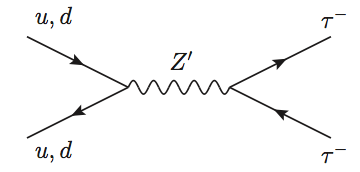
\includegraphics[width=0.4\textwidth]{figures/ZprimeToTauTau.png}
  \caption{\label{fig:ZprimeToTauTau} $Z^\prime \to \tau\tau$ event at the LHC, wherein two quarks from colliding protons form a $Z^\prime$ which then decays to an oppositely-charged, back-to-back pair of $\tau$ leptons.}
\end{figure}

\section{Models Predicting New Neutral Bosons}

\subsection{Sequential Standard Model (SSM)}

The SSM does not predict the existence of a $Z^{\prime}$ due to a larger symmetry group, but rather manually adds an extra neutral gauge boson, $Z^{\prime}_{SSM}$, which is identical to the SM $Z$, with the same couplings to quarks and leptons. This model is not gauge invariant unless the $Z^{\prime}_{SSM}$ couples to additional, exotic fermions or unless it exists as an excitation of the SM $Z$ in the case of models involving extra dimensions at the weak scale. Its decay width is given by 
\begin{equation}
\Gamma_{Z^{\prime}} = \Gamma_Z \times M_{Z^{\prime}}/M_{Z}.
\end{equation}
\noindent While the SSM is typically not gauge-invariant, it still serves as an exceptionally useful benchmark in the search for new physics, as it can be used as a baseline for comparison with other models should an excess be observed.\cite{SSM} Given this, the $Z^{\prime}_{SSM}$ is the chief signal used in the physics searches described in this thesis.

\subsection{Grand Unified Theory (GUT)-inspired Models}

Models that try to merge the strong and electroweak interactions into one larger, all-encompassing symmetry group are called Grand Unified Theories (GUTs). One popular GUT is called $E_6$ and takes its name from the set of symmetry groups selected as candidates for one such larger group. In the $E_6$ model, the $E_6$ groups break in the following fashion:
\begin{equation}
E_6 \to SO(10) \times U(1)_\psi \to SU(5) \times U(1)_\chi \times U(1)_\psi \to SM \times U(1)_{\theta_{E_6}}.
\end{equation}

\noindent The new gauge boson ($Z^\prime$ candidate) is predicted to arise as a mixing of the $U(1)_\psi$ and $U(1)_\chi$ groups with a mixing angle $\theta_{E_6}$:

\begin{equation}
Z^{\prime} = Z^\prime_\chi \cos{\theta_{E_6}} + Z^\prime_\psi \sin{\theta_{E_6}}.
\end{equation}

$\theta_{E_6}$ is a free parameter ranging from $-90^{\deg}$ to $90^{\deg}$. The choice of $\theta_{E_6}$ is dictated by the model, and the four most popular values are $\theta_{E_6} = 0^{\deg}$ ($Z^\prime_\chi$), $\theta_{E_6} = 90^{\deg}$ ($Z^\prime_\psi$), $\theta_{E_6} = \arcsin{\sqrt{3/8}}$ ($Z^\prime_\eta$), and $\theta_{E_6} = \arcsin{\sqrt{5/8}}$ ($Z^\prime_I$).\cite{E6} While these $E_6$-inspired models were not included in the 13 TeV search, the $Z^\prime_\psi$ signal was one of the principal signal Monte Carlo samples used in the 8 TeV analysis.